\chapter{Test-Time Training (TTT): Tent, MIM, CoTTA, EATA, SAR}

\ChapterMeta{
This chapter explains controlled test-time adaptation (Tent/MIM/CoTTA/EATA/SAR), presets, guard rails, and reset policies for fair comparisons.
}{
It can improve robustness under domain shift by adapting weights in memory, while keeping cost bounded and results reproducible.
}{
It is most relevant when there is clear domain shift; comparisons require fixed image sets, bounded \cmd{--ttt-max-batches}, and careful seed and reset policy control.
}
\ChapterAudience{Read this chapter when you are adapting models under domain shift and want a method-by-method guide to Tent, MIM, CoTTA, EATA, and SAR.}

\paragraph{Readiness classification.}
TTT is a \textbf{research-oriented} lane in \yolozu{}.
Use it as an inference-time adaptation mode with bounded cost and explicit review, not as the default production update loop.
See \path{docs/production_readiness.md}.


\section{Scope and support}
\yolozu{} supports controlled test-time training (TTT) for the \path{rtdetr_pose} adapter via
\path{tools/export_predictions.py} or the unified wrapper \path{tools/yolozu.py}.

Authoritative references:
\begin{itemize}
  \item \path{docs/ttt_protocol.md}
  \item \path{docs/ttt_integration_plan.md}
  \item \path{docs/mim_inference.md}
\end{itemize}

TTT updates weights \emph{in memory} using unlabeled test data before (or during) inference \cite{sun2020ttt,wang2021tent}.
This makes comparisons sensitive to domain shift, random seeds, and reset policy.

\subsection{Plain-language glossary for this chapter}
Many readers first get stuck not on the code, but on the names. The short
meanings below are enough to read the rest of this chapter:
\begin{itemize}
  \item \textbf{TTA} (\textbf{Test-Time Augmentation}): run inference several times on simple transformed versions of the same image, then merge the predictions. This does \emph{not} update model weights.
  \item \textbf{TTT} (\textbf{Test-Time Training}): update some model parameters in memory at inference time using unlabeled test data.
  \item \textbf{CTTA} (\textbf{Continual Test-Time Adaptation}): a streaming form of TTT where adaptation continues over many incoming batches instead of resetting after every image.
  \item \textbf{LoRA}: a small trainable adapter added to selected layers, used when you want limited, safer parameter updates instead of moving the full model.
  \item \textbf{Norm-only update}: adapt only normalization-layer affine parameters (for example BatchNorm or LayerNorm scale/bias). This is one of the safest update scopes.
  \item \textbf{EMA} (\textbf{Exponential Moving Average}): a smoothed teacher copy of model weights. It changes more slowly than the student and is often used to stabilize adaptation.
  \item \textbf{Reset policy}: when and how the adapted weights are restored. \cmd{sample} means ``reset after each image/subset''; \cmd{stream} means ``carry updates forward across the stream.''
  \item \textbf{Guard rail}: a safety rule that limits adaptation, for example restricting which parameters may update or stopping updates when sample selection looks unreliable.
\end{itemize}

\paragraph{What the method names mean at a glance.}
\begin{itemize}
  \item \textbf{Tent}: minimize prediction entropy so the model becomes more confident on shifted inputs.
  \item \textbf{MIM}: use a masked-reconstruction objective so the model must infer hidden structure, not only sharpen confidence.
  \item \textbf{CoTTA}: a continual TTT method that combines student updates, an EMA-style teacher, augmentation agreement, and partial restoration so the model does not drift too far.
  \item \textbf{EATA}: an efficiency/reliability-oriented TTT method that adapts only on selected samples instead of updating on everything.
  \item \textbf{SAR}: a sharpness-aware robustness method; in practical terms, it tries to adapt in directions that are locally more stable instead of overreacting to noisy gradients.
\end{itemize}

\paragraph{How to read the rest of the chapter.}
If you only want the shortest reading path, use this order:
\begin{enumerate}
  \item understand whether you need \textbf{TTA} or \textbf{TTT},
  \item understand the \textbf{update scope} (norm-only, LoRA, or full-model),
  \item then compare the methods (Tent, MIM, CoTTA, EATA, SAR).
\end{enumerate}
This order matters because many failures blamed on the method are actually
caused by an overly broad update scope or an unsafe reset policy.

\subsection{Operator quick guide (read first)}
\begin{itemize}
  \item \textbf{Default OFF}: TTT is opt-in and only activates when \cmd{--ttt} is set.
  \item \textbf{Default update scope}: start with safe presets (norm-only / adapter-safe). For CoTTA/EATA/SAR rollout, keep updates constrained to LoRA/Norm-safe subsets first.
  \item \textbf{Reset recommendation}: for controlled comparisons, prefer \cmd{--ttt-reset sample}; for streaming latency operation, use bounded \cmd{--ttt-reset stream} with explicit \cmd{--ttt-max-batches}.
\end{itemize}

\begin{figure}[h]
\centering
\resizebox{0.95\linewidth}{!}{%
\begin{tikzpicture}[
  node distance=10mm,
  font=\small,
  box/.style={draw, rounded corners, align=left, inner sep=6pt},
  arrow/.style={-{Latex[length=2mm]}, thick}
]

\node[box] (all) {\textbf{Model parameters}\\(backbone + encoder + heads)};
\node[box, below=10mm of all] (filter) {\textbf{Update filter}\\(\cmd{--ttt-update-filter})};

\node[box, below=12mm of filter, xshift=-40mm] (norm) {\textbf{norm-only}\\(BN/LN/GN affine)};
\node[box, below=12mm of filter] (lora) {\textbf{LoRA-only}\\(low-rank adapters)};
\node[box, below=12mm of filter, xshift=40mm] (full) {\textbf{full-model}\\(avoid by default)};

\draw[arrow] (all) -- (filter);
\draw[arrow] (filter) -- (norm);
\draw[arrow] (filter) -- (lora);
\draw[arrow] (filter) -- (full);

\end{tikzpicture}
}
\caption{TTT update scope: start with constrained update filters (norm/LoRA) and keep full-model updates opt-in.}
\end{figure}

\section{When TTT is meaningful}
On clean COCO-style validation, TTT can be neutral or harmful.
To demonstrate improvements, you typically need a clear domain shift (e.g., corruptions, style shift, different camera).

Practical baseline:
\begin{itemize}
  \item Baseline domain: clean COCO \cmd{val2017}
  \item Target domain: shifted dataset or corrupted copy of COCO images
\end{itemize}

\subsection{Deterministic shift-target recipe}
For reproducible TTT evidence, generate a deterministic corrupted target split with:
\begin{lstlisting}[language=bash]
python3 scripts/prepare_ttt_domain_shift_target.py \
  --dataset-root data/smoke \
  --split val \
  --out reports/domain_shift/smoke_gaussian_blur_s2 \
  --corruption gaussian_blur \
  --severity 2 \
  --seed 2026 \
  --force
\end{lstlisting}

This produces \path{domain_shift_recipe.json} containing
\path{export_settings.domain_shift_target} with fixed
(\texttt{corruption}, \texttt{severity}, \texttt{seed}, \texttt{images\_sha256}).

To bind that recipe into prediction artifacts:
\begin{lstlisting}[language=bash]
python3 tools/export_predictions.py \
  --adapter dummy \
  --dataset reports/domain_shift/smoke_gaussian_blur_s2 \
  --split val \
  --wrap \
  --domain-shift-recipe reports/domain_shift/smoke_gaussian_blur_s2/domain_shift_recipe.json \
  --output reports/pred_shift_target.json
\end{lstlisting}

With \cmd{--wrap}, outputs explicitly include:
\begin{itemize}
  \item \path{meta.export_settings.domain_shift_target}
  \item \path{meta.export_settings.domain_shift_recipe} (\texttt{path}, \texttt{sha256})
\end{itemize}

\subsection{Real result summary: use this first}
The first thing beginners need is not a noisy overlay, but a controlled \emph{result summary}.
Figure~\ref{fig:ttt-real-summary} is therefore the primary onboarding figure for this chapter.
It uses the same few-shot checkpoint, the same ten shifted images, and the same seed for every method.
That means the bar chart is a controlled comparison, not a one-off anecdote.
The checked-in PNG figures are regenerated with \path{tools/render_ttt_manual_figures.py}.

Command summary (deterministic target + same checkpoint, with and without TTT):
\begin{lstlisting}[language=bash]
# 1) Prepare a deterministic shifted target split (1 image for illustration).
python3 scripts/prepare_ttt_domain_shift_target.py \
  --dataset-root data/smoke \
  --split val \
  --out reports/domain_shift/smoke_gaussian_blur_s3_1img \
  --corruption gaussian_blur \
  --severity 3 \
  --seed 2026 \
  --max-images 1 \
  --force

# 2) Inference overlays without TTT (torch backend + small repo-shipped checkpoint).
python3 tools/yolozu.py predict-images \
  --backend torch --device cpu \
  --config rtdetr_pose/configs/base.json \
  --checkpoint reports/rtdetr_pose_ckpt_coco128_gpu_matcher.pt \
  --image-size 320 --score-threshold 0.05 --max-detections 20 \
  --input-dir reports/domain_shift/smoke_gaussian_blur_s3_1img/images/val \
  --max-images 1 \
  --overlays-dir reports/ttt_demo/no_ttt_overlays \
  --output reports/ttt_demo/pred_no_ttt.json \
  --force

# 3) Same inference but with TTT enabled (Tent safe preset, reset per sample).
python3 tools/yolozu.py predict-images \
  --backend torch --device cpu \
  --config rtdetr_pose/configs/base.json \
  --checkpoint reports/rtdetr_pose_ckpt_coco128_gpu_matcher.pt \
  --image-size 320 --score-threshold 0.05 --max-detections 20 \
  --input-dir reports/domain_shift/smoke_gaussian_blur_s3_1img/images/val \
  --max-images 1 \
  --overlays-dir reports/ttt_demo/ttt_overlays \
  --output reports/ttt_demo/pred_ttt.json \
  --ttt --ttt-preset safe --ttt-reset sample --ttt-seed 2026 \
  --ttt-log-out reports/ttt_demo/ttt_log.json \
  --force
\end{lstlisting}

\begin{figure}[htbp]
  \centering
  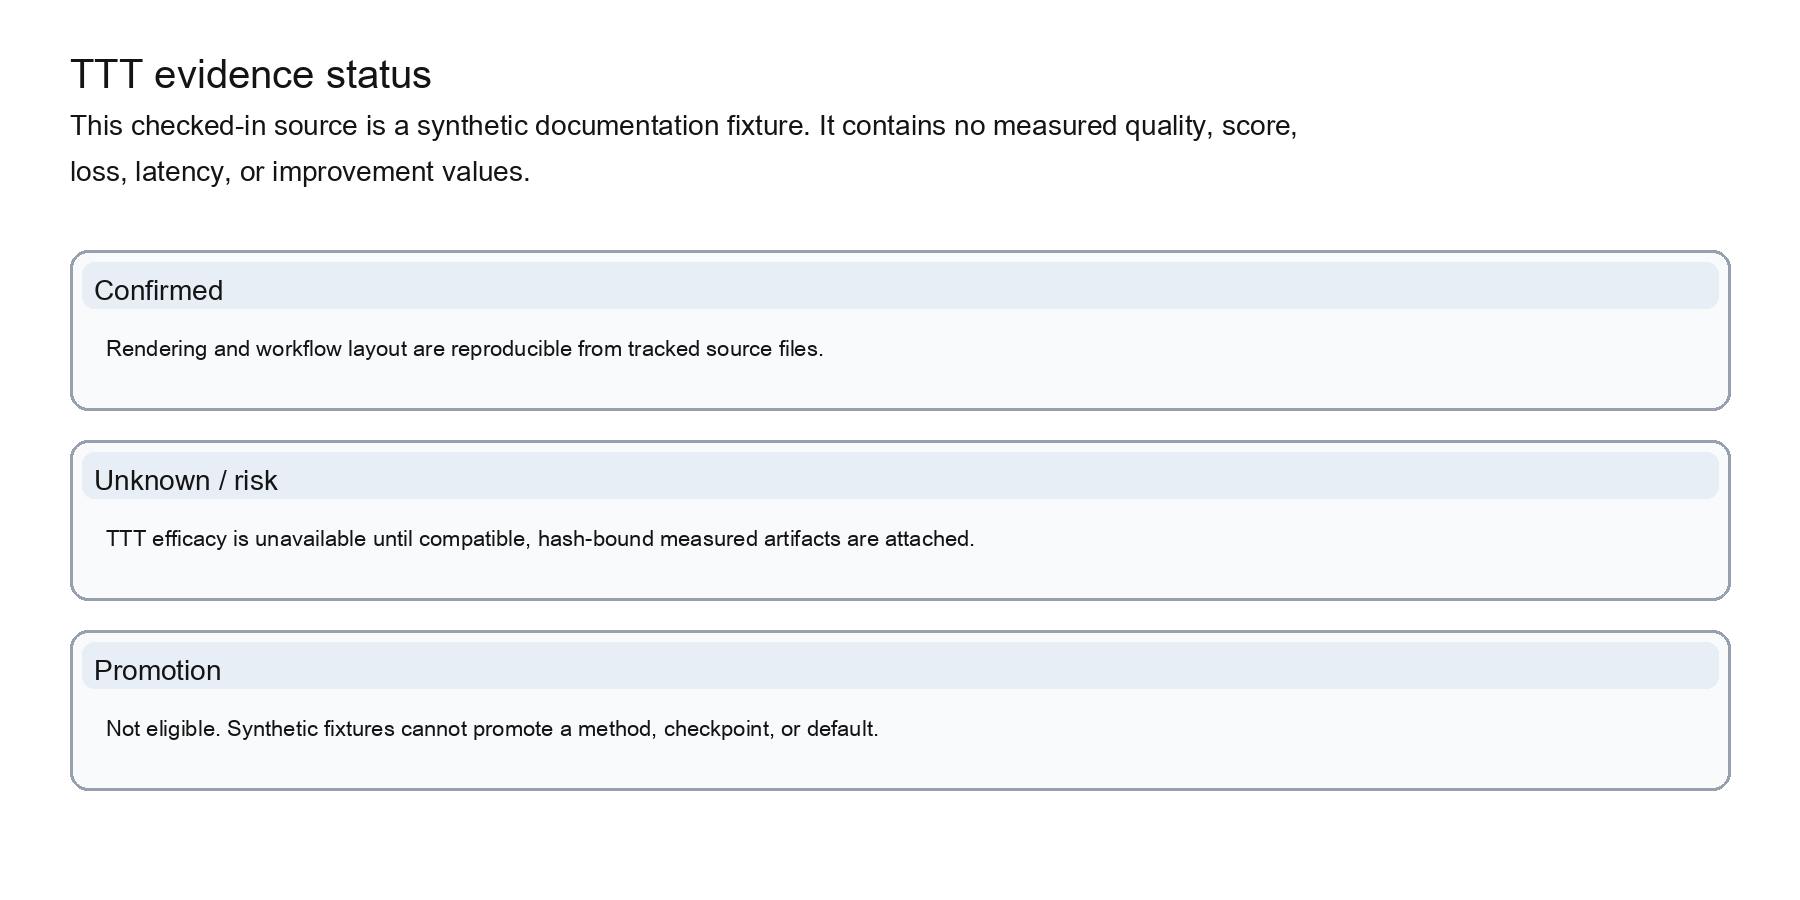
\includegraphics[width=\textwidth]{figures/ttt_method_results_summary.png}
  \caption{Primary TTT result figure. Real fixed-subset result summary from the ten-image shifted probe in \texttt{reports/ttt\_improvement\_probe}. Tent, CoTTA, EATA, and SAR all improve from \texttt{map50=0.00326797} to \texttt{0.00392157} and from \texttt{map50\_95=0.000326797} to \texttt{0.000392157} under the same checkpoint, subset, and seed. MIM is shown separately as execution evidence because the current repo-backed MIM smoke fixture proves the masked-reconstruction path runs (\texttt{steps\_run=2}, \texttt{mean\_final\_loss=0.461853}) but does not change exported detections on its tiny two-image smoke subset.}
  \label{fig:ttt-real-summary}
\end{figure}

\begin{figure}[htbp]
  \centering
  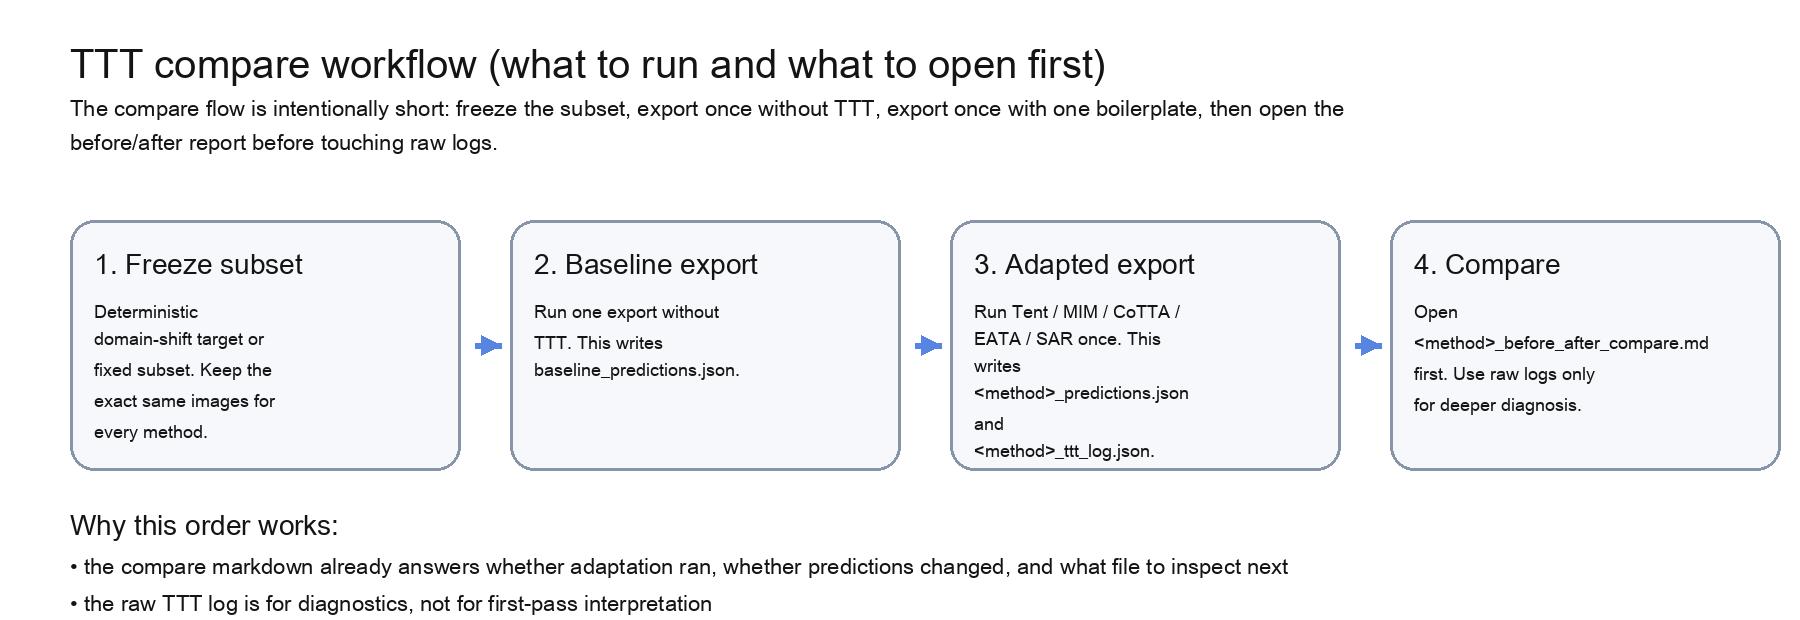
\includegraphics[width=\textwidth]{figures/ttt_compare_pipeline.png}
  \caption{Beginner-oriented processing flow for every TTT/CTTA method. Freeze the subset, export once without TTT, export once with one boilerplate, then open \texttt{<method>\_before\_after\_compare.md} before reading raw logs. This is the recommended reading order because the compare markdown answers whether adaptation actually ran, whether predictions changed, and which artifact to inspect next.}
  \label{fig:ttt-compare-workflow}
\end{figure}

\subsection{Metric micro-demo: show a delta (recommended)}
The visual example above shows \emph{what changes}. For onboarding and regression checks, it is also useful to show
\emph{a small metric delta} on a deterministic shift target.

\yolozu{} provides a self-contained micro-demo that:
\begin{itemize}
  \item trains a tiny few-shot checkpoint on clean \path{data/smoke} first (so no external weights download is required),
  \item applies a deterministic corruption to create a shifted target split,
  \item evaluates a simple mAP proxy for \textbf{no TTT} vs \textbf{with TTT} (and writes overlay PNGs).
\end{itemize}

\begin{lstlisting}[language=bash,caption={TTT improvement micro-demo: few-shot train + deterministic shift + metric delta.}]
# pip users:
python3 -m pip install -U 'yolozu[demo]'
yolozu demo ttt

# repo checkout equivalent:
python3 tools/yolozu.py demo ttt
\end{lstlisting}

Outputs include:
\begin{itemize}
  \item \path{demo_output/ttt/<utc>/ttt_improvement_report.json} (with \path{metrics.delta}),
  \item \path{demo_output/ttt/<utc>/overlay_no_ttt.png} and \path{overlay_ttt.png}.
\end{itemize}

Example stdout (CPU, deterministic seeds; values are intentionally tiny, the point is the reproducible delta):
\begin{itemize}
  \item \texttt{map50 0.00326797 $\to$ 0.00392157}
  \item \texttt{map50\_95 0.000326797 $\to$ 0.000392157}
\end{itemize}

\subsection{Per-image probe grid: concrete, but still secondary to the metric chart}
Figure~\ref{fig:ttt-qualitative-panel} uses the same fixed ten-image shifted subset as the metric summary.
It is intentionally secondary. The goal of this figure is not to prove quality with a single image, but to make the result concrete:
for each shifted image, it shows the top baseline detection, the top TTT detection, and the score movement.
This makes it much easier to explain what the detector is trying to localize and how the prediction changed, while the actual proof of improvement still comes from Figure~\ref{fig:ttt-real-summary}.

\begin{figure}[htbp]
  \centering
  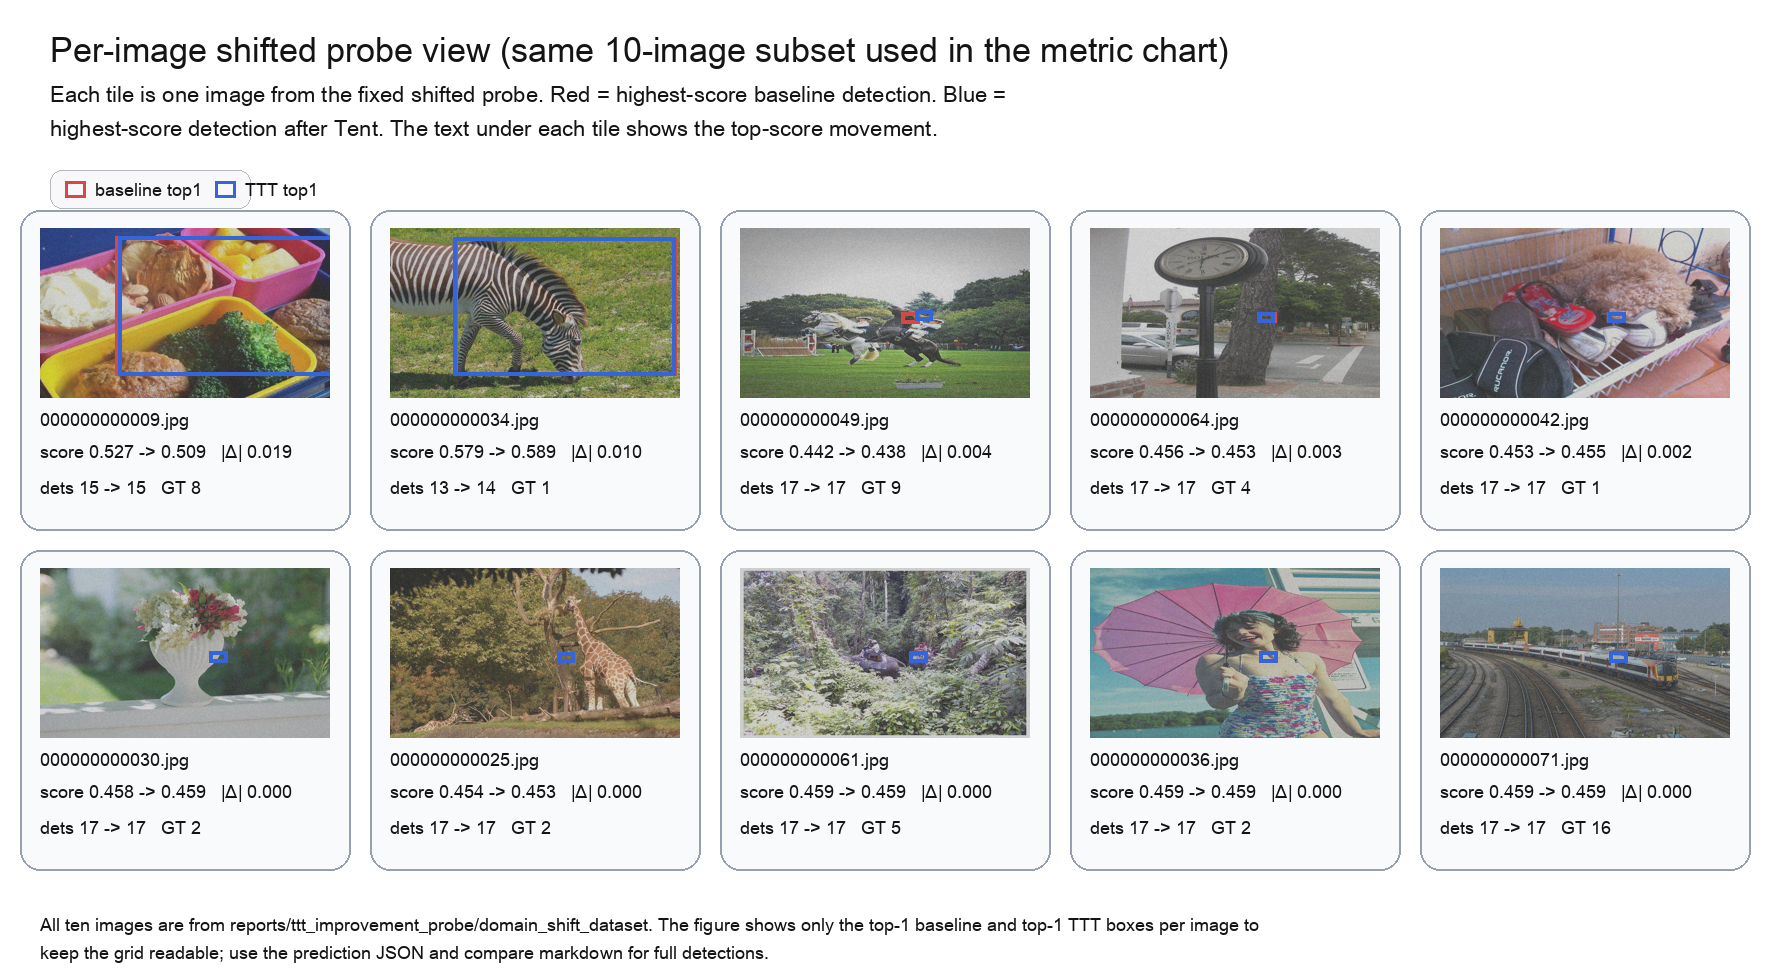
\includegraphics[width=\textwidth]{figures/ttt_probe_example_panel.png}
  \caption{Per-image result grid from the same fixed ten-image shifted probe used in Figure~\ref{fig:ttt-real-summary}. Each tile is one actual shifted image. Red marks the highest-score baseline detection without TTT; blue marks the highest-score detection after Tent. The text under each tile reports the top-score movement plus detection-count and ground-truth counts. This figure answers ``what was the detector trying to localize, and how did the top detection move on each image?'' The quantitative claim still comes from the fixed-subset metric chart in Figure~\ref{fig:ttt-real-summary}.}
  \label{fig:ttt-qualitative-panel}
\end{figure}

\section{Presets (start here)}
Both CLIs expose \cmd{--ttt-preset}:
\begin{itemize}
  \item \cmd{safe}: Tent + BN-affine only (\cmd{update_filter=norm_only})
  \item \cmd{adapter_only}: Tent + adapter/head only
  \item \cmd{mim_safe}: MIM + adapter/head only
  \item \cmd{cotta_safe}: CoTTA with conservative update/restore guard rails
  \item \cmd{eata_safe}: EATA selective adaptation with anti-forgetting defaults
  \item \cmd{sar_safe}: SAR LoRA-first sharpness-aware adaptation defaults
  \item \cmd{pose_safe}/\cmd{keypoints_safe}/\cmd{depth_safe}/\cmd{seg_safe}: task-aware Tent defaults
  \item \cmd{pose_mim}: pose-aware MIM defaults
\end{itemize}

Presets override core knobs (method, steps, lr, update filter, max batches) and set conservative guard rails unless you override them.
Use \cmd{--ttt-sdft-task \{pose,keypoints,depth,seg,full\}} and \cmd{--ttt-aux-*} weights to steer multi-task adaptation losses.

\section{Algorithm catalog with concrete examples}
The currently implemented parameter-updating TTT/CTTA methods are:
\cmd{tent}, \cmd{mim}, \cmd{cotta}, \cmd{eata}, and \cmd{sar}.
In practice, the fastest way to compare them fairly is:
\begin{enumerate}
  \item freeze the image subset,
  \item run the same adapter/checkpoint on the same shifted images,
  \item emit wrapped predictions for each method,
  \item compare method-specific logs and benchmark artifacts.
\end{enumerate}

\subsection{Recommended operator workflow: boilerplate compare}
Instead of retyping a long raw export command for each method, use the boilerplate compare wrapper:

\begin{lstlisting}[language=bash]
bash scripts/ttt_compare.sh \
  --boilerplate tent \
  --dataset data/smoke \
  --split val \
  --checkpoint /path/to.ckpt \
  --run-dir reports/ttt_compare/tent \
  --device cuda
\end{lstlisting}

This workflow writes:
\begin{itemize}
  \item \path{plan.json}
  \item \path{baseline_predictions.json}
  \item \path{<method>_predictions.json}
  \item \path{<method>_ttt_log.json}
  \item \path{<method>_before_after_compare.json}
  \item \path{<method>_before_after_compare.md}
\end{itemize}

The compare report provides the actual \textbf{before/after} summary:
baseline vs adapted prediction counts, TTT loss/runtime summary, and a compact drift summary
(\texttt{changed\_images}, \texttt{missing\_match\_failures}, \texttt{value\_mismatch\_failures}).

\subsection{Which files to compare for each method}
\begin{center}
\begin{tabular}{p{2.0cm} p{2.2cm} p{3.1cm} p{3.1cm} p{3.4cm}}
\toprule
\textbf{Method} & \textbf{Boilerplate} & \textbf{Baseline} & \textbf{Adapted} & \textbf{Primary before/after artifact} \\
\midrule
Tent & \cmd{tent} & \path{reports/ttt_compare/tent/baseline_predictions.json} & \path{reports/ttt_compare/tent/tent_predictions.json} & \path{reports/ttt_compare/tent/tent_before_after_compare.md} \\
MIM & \cmd{mim} & \path{reports/ttt_compare/mim/baseline_predictions.json} & \path{reports/ttt_compare/mim/mim_predictions.json} & \path{reports/ttt_compare/mim/mim_before_after_compare.md} \\
CoTTA & \cmd{cotta} & \path{reports/ttt_compare/cotta/baseline_predictions.json} & \path{reports/ttt_compare/cotta/cotta_predictions.json} & \path{reports/ttt_compare/cotta/cotta_before_after_compare.md} \\
EATA & \cmd{eata} & \path{reports/ttt_compare/eata/baseline_predictions.json} & \path{reports/ttt_compare/eata/eata_predictions.json} & \path{reports/ttt_compare/eata/eata_before_after_compare.md} \\
SAR & \cmd{sar} & \path{reports/ttt_compare/sar/baseline_predictions.json} & \path{reports/ttt_compare/sar/sar_predictions.json} & \path{reports/ttt_compare/sar/sar_before_after_compare.md} \\
\bottomrule
\end{tabular}
\end{center}

Recommended reading order:
\begin{enumerate}
  \item \path{plan.json} to confirm the frozen subset and boilerplate,
  \item \path{<method>\_before\_after\_compare.md} for the compact summary,
  \item \path{<method>\_ttt\_log.json} for adaptation loss/runtime details,
  \item method-specific follow-up tools only when deeper diagnostics are needed.
\end{enumerate}

\textbf{Important note.}
The shipped \cmd{mim} and \cmd{sar} boilerplates expand the safe defaults
directly and force
\cmd{--ttt-update-filter norm_only} so they run against the repo-shipped
checkpoint without requiring LoRA-specific weights. If a team owns a dedicated
adapter/LoRA checkpoint, it is better to copy the JSON boilerplate and switch
the update filter there than to fall back to a long raw CLI invocation.
The \cmd{mim} boilerplate also injects the repo-backed config
\path{configs/examples/ttt_compare/rtdetr_pose_mim_compare.json} into both the
baseline and adapted export commands so the MIM branch is enabled without a
manual config override.

\subsection{Smoke compare snapshot (repo-shipped checkpoint)}
We also validated the boilerplates against the repo-shipped checkpoint
\path{reports/rtdetr_pose_ckpt_coco128_gpu_matcher.pt} on \path{data/smoke},
\cmd{split=val}, \cmd{max-images=2}, \cmd{device=cpu}, with \cmd{--skip-eval}.

This is a workflow validation snapshot, not a quality claim. The tiny smoke
subset produced zero detections in both baseline and adapted runs, so the
useful signal here is method completion and the TTT log behavior.

\begin{table}[htbp]
\centering
\begin{tabular}{p{1.8cm} p{3.8cm} p{2.6cm} p{1.3cm} p{1.8cm}}
\toprule
\textbf{Method} & \textbf{Run dir} & \textbf{Real compare status} & \textbf{Steps} & \textbf{Mean final loss} \\
\midrule
Tent & \path{reports/ttt_compare/tent_smoke_cpu} & completed & 2 & 4.214431 \\
MIM & \path{reports/ttt_compare/mim_smoke_cpu} & completed & 2 & 0.461853 \\
CoTTA & \path{reports/ttt_compare/cotta_smoke_cpu} & completed & 1 & 4.243579 \\
EATA & \path{reports/ttt_compare/eata_smoke_cpu} & completed & 0 & null \\
SAR & \path{reports/ttt_compare/sar_smoke_cpu} & completed & 2 & 4.211009 \\
\bottomrule
\end{tabular}
\caption{Smoke compare snapshot for the repo-shipped checkpoint on \texttt{data/smoke}, \cmd{split=val}, \cmd{max-images=2}, \cmd{device=cpu}, with \cmd{--skip-eval}. This is a workflow-validation table, not a quality leaderboard. Warning notes are intentionally moved out of the table for readability: MIM uses the repo-backed compare config \texttt{configs/examples/ttt\_compare/rtdetr\_pose\_mim\_compare.json}; EATA reports \cmd{eata\_empty\_selected\_set} on both smoke images; Tent, CoTTA, and SAR complete without warnings on this smoke subset.}
\end{table}

For the completed runs, the compact summaries are:
\begin{itemize}
  \item \path{reports/ttt_compare/tent_smoke_cpu/tent_before_after_compare.md}
  \item \path{reports/ttt_compare/mim_smoke_cpu/mim_before_after_compare.md}
  \item \path{reports/ttt_compare/cotta_smoke_cpu/cotta_before_after_compare.md}
  \item \path{reports/ttt_compare/eata_smoke_cpu/eata_before_after_compare.md}
  \item \path{reports/ttt_compare/sar_smoke_cpu/sar_before_after_compare.md}
\end{itemize}

\subsection{How to read the smoke compare table}
The smoke table above is a \textbf{workflow validation table}. It tells you whether the method ran safely and emitted reproducible artifacts. It does \emph{not} claim that one method is globally better than another.

Read the columns in this order:
\begin{enumerate}
  \item \textbf{Real compare status}: did the whole compare workflow finish?
  \item \textbf{Steps}: how many adaptation updates actually ran?
  \item \textbf{Mean final loss}: what was the final adaptation objective value?
\end{enumerate}

Two common beginner mistakes:
\begin{itemize}
  \item treating \cmd{mean\_final\_loss} as a quality score across methods,
  \item treating \cmd{steps=0} as a failure.
\end{itemize}
Warning notes are now kept in the table caption rather than in a dedicated wide column.
For example, EATA can legitimately report \cmd{steps=0} with
\cmd{eata\_empty\_selected\_set}. That means the method decided \emph{not} to adapt on those smoke images, which is conservative behavior, not a crash.

\begin{figure}[h]
\centering
\resizebox{0.97\linewidth}{!}{%
\begin{tikzpicture}[
  node distance=8mm,
  font=\small,
  box/.style={draw, rounded corners, align=center, inner sep=6pt, minimum width=24mm, fill=white},
  note/.style={align=center, font=\scriptsize, fill=white, inner sep=1pt},
  arrow/.style={-{Latex[length=2mm]}, thick}
]
\node[box] (input) {\textbf{Shifted input}\\blur / style shift};
\node[box, right=10mm of input] (base) {\textbf{Baseline predict}\\no update};
\node[box, right=10mm of base] (adapt) {\textbf{Adapt}\\run Tent / MIM / CoTTA / EATA / SAR};
\node[box, right=10mm of adapt] (pred) {\textbf{Adapted predict}\\same subset};
\node[box, right=10mm of pred] (cmp) {\textbf{Compare}\\before vs after};
\node[note] (sameimg) at ($(base.east)!0.5!(adapt.west)+(0,4mm)$) {same images};
\node[note] (weights) at ($(adapt.east)!0.5!(pred.west)+(0,4mm)$) {weights updated in memory};
\begin{pgfonlayer}{bg}
\draw[arrow] (input) -- (base);
\draw[arrow] (base) -- (adapt);
\draw[arrow] (adapt) -- (pred);
\draw[arrow] (pred) -- (cmp);
\end{pgfonlayer}
\end{tikzpicture}
}
\caption{Common TTT workflow in \yolozu{}: run the baseline and the adapted variant on the same deterministic image subset, then compare their artifacts.}
\end{figure}

\subsection{Operator workflow: what to do first}
For every method, the safest operator workflow is:
\begin{enumerate}
  \item choose a fixed dataset subset or a deterministic domain-shift target,
  \item run \path{scripts/ttt_compare.sh} with one boilerplate,
  \item open \path{<method>\_before\_after\_compare.md},
  \item only then inspect \path{<method>\_ttt\_log.json}.
\end{enumerate}

This order matters. The compare markdown is the onboarding artifact. It answers the first three questions operators usually have:
\begin{itemize}
  \item Did adaptation actually run?
  \item Did predictions change?
  \item Which file should I inspect next?
\end{itemize}

\subsection{Tent}
\textbf{What the name means.}
Tent is short for \textbf{fully Test-time adaptation by ENTropy minimization}.
The name is useful because it already tells you the two essential ideas:
\begin{itemize}
  \item adaptation happens at \emph{test time},
  \item entropy is the signal being minimized.
\end{itemize}

\textbf{Principle.}
Tent minimizes prediction entropy online using a restricted parameter subset \cite{wang2021tent}. In plain language, it pushes the model toward making sharper, more confident predictions on shifted inputs, but only lets a small subset of parameters move.

\textbf{What entropy means here.}
If a prediction spreads probability mass across many classes, the entropy is high.
If the same prediction becomes concentrated on one class, the entropy is low.
For a single prediction vector $p$, the usual entropy term is:
\[
H(p) = - \sum_c p_c \log p_c.
\]
Tent adapts a small subset of parameters by reducing the average prediction entropy over the selected test-time samples:
\[
\min_{\theta_{\mathrm{adapt}}} \; \mathrm{E}_{x \sim \mathrm{test\ stream}} \left[ H\!\left(p_{\theta}(y \mid x)\right) \right].
\]
In \yolozu{}'s safe presets, $\theta_{\mathrm{adapt}}$ is intentionally small, usually norm-affine parameters or a restricted adapter/head subset.

\textbf{Why it can work.}
Under mild domain shift, the model often still attends to roughly the right object, but its output distribution becomes softer and less decisive.
Tent exploits that situation: it does not ask the model to discover a brand-new concept, it only asks whether a more confident local decision boundary gives a better answer.

\textbf{What it is not.}
\begin{itemize}
  \item It is not supervised fine-tuning.
  \item It does not tell the model which class is correct.
  \item It assumes ``become more confident'' is a useful direction on the current shifted sample.
\end{itemize}

\begin{figure}[h]
\centering
\resizebox{0.95\linewidth}{!}{%
\begin{tikzpicture}[
  node distance=8mm,
  font=\small,
  box/.style={draw, rounded corners, align=center, inner sep=6pt},
  arrow/.style={-{Latex[length=2mm]}, thick}
]
\node[box] (x) {Shifted image};
\node[box, right=10mm of x] (p) {Prediction distribution};
\node[box, right=10mm of p] (h) {Entropy loss};
\node[box, right=10mm of h] (u) {Update norm / affine parameters};
\draw[arrow] (x) -- (p);
\draw[arrow] (p) -- (h);
\draw[arrow] (h) -- (u);
\end{tikzpicture}
}
\caption{Tent: use prediction entropy as the adaptation signal and keep updates constrained to a safe parameter subset.}
\end{figure}

\textbf{When to use it.}
Tent is the best first method. Choose it when you want the smallest operational jump away from baseline inference and the easiest debug path.

\textbf{Concrete procedure.}
\begin{lstlisting}[language=bash]
bash scripts/ttt_compare.sh \
  --boilerplate tent \
  --dataset data/smoke \
  --split val \
  --checkpoint /path/to.ckpt \
  --run-dir reports/ttt_compare/tent \
  --device cuda
\end{lstlisting}

\textbf{How to read the result.}
\begin{itemize}
  \item Open \path{tent\_before\_after\_compare.md} first.
  \item Check whether \cmd{steps\_run > 0}.
  \item If \cmd{changed\_images=0}, adaptation completed but exported predictions did not change on this subset.
  \item Open \path{tent\_ttt\_log.json} only if you need guard or runtime detail.
\end{itemize}

\textbf{Concrete repo result.}
On the fixed ten-image shifted probe in Figure~\ref{fig:ttt-real-summary}, Tent improves
\texttt{map50} from \texttt{0.00326797} to \texttt{0.00392157} and
\texttt{map50\_95} from \texttt{0.000326797} to \texttt{0.000392157}.
The effect is small, but it is reproducible under the same checkpoint, subset, and seed.

\textbf{Pros.}
\begin{itemize}
  \item easiest method to explain,
  \item cheapest adaptation cost,
  \item safest default when using norm-only updates.
\end{itemize}

\textbf{Cons.}
\begin{itemize}
  \item weakest self-supervised signal,
  \item can sharpen wrong predictions under severe shift,
  \item often less expressive than reconstruction-based methods.
\end{itemize}

\subsection{MIM}
\textbf{What the name means.}
MIM stands for \textbf{Masked Image Modeling}.
In plain language, we deliberately hide part of the visual signal and ask the model to reconstruct or predict what is missing.
That is why MIM feels more structural than Tent: it is not only asking for confidence, it is asking for internal consistency.

\textbf{Principle.}
MIM uses masked reconstruction and optional entropy terms to adapt from unlabeled shifted inputs. Instead of only asking the model to become more confident, it also asks the model to reconstruct hidden structure from partially masked internal features. The lineage is broader than MAE alone: denoising autoencoders already used corruption-plus-reconstruction as a representation-learning signal in 2008 \cite{vincent2008dae}, image inpainting-style reconstruction was used as a visual self-supervised task in Context Encoders \cite{pathak2016context}, and modern masked-image-modeling references include Masked Autoencoders (MAE) \cite{he2022mae} and SimMIM \cite{xie2022simmim}. For direct test-time usage, representative references are Test-Time Training with Masked Autoencoders \cite{gandelsman2022tttmae} and TTT-MIM \cite{mansour2024tttmim}. \yolozu{} uses this family of masked-image-modeling ideas as an inference-time auxiliary signal rather than as a standalone pretraining recipe.

\textbf{Minimal objective view.}
Let $M$ denote a mask and $R_{\theta}$ denote the reconstruction path.
A simplified masked-reconstruction loss can be written as:
\[
L_{\mathrm{MIM}} = \left\| R_{\theta}\!\left((1-M)\odot x\right) - M \odot x \right\|.
\]
Many practical test-time variants combine this reconstruction term with an entropy term:
\[
L_{\mathrm{adapt}} = \lambda_{\mathrm{mim}} L_{\mathrm{MIM}} + \lambda_{\mathrm{ent}} H\!\left(p_{\theta}(y \mid x)\right).
\]
The exact target differs across implementations, but the operational story stays the same:
\begin{itemize}
  \item hide part of the signal,
  \item ask the model to infer the hidden structure,
  \item use that self-supervised error as the adaptation signal.
\end{itemize}

\textbf{Research lineage and IP note.}
This manual cites representative prior-art waypoints so that operators can place the method in a broader technical lineage instead of treating MIM-style adaptation as a single new idea. The broad pattern---corrupt or mask part of the input/feature state, reconstruct hidden structure, and use that self-supervised loss to improve robustness---predates the current wording of test-time masked adaptation. This note is meant to support technical due diligence and prior-art positioning only; it is \textbf{not} legal advice and it is \textbf{not} a non-infringement opinion. Any deployment-specific IP or patent review belongs to qualified counsel.

\textbf{Why it can work.}
Entropy-only adaptation can be too weak when the shift is geometric, structural, or pose-sensitive.
MIM adds a denser self-supervised objective: the model is rewarded not merely for being decisive, but for reconstructing a plausible hidden structure from incomplete evidence.
That is why MIM is often easier to justify in pose-heavy workflows than plain confidence sharpening.

\textbf{What it is not.}
\begin{itemize}
  \item It is not just ``MAE pretraining at inference time''.
  \item It is not guaranteed to improve every exported detection.
  \item It is usually more model-specific than Tent because the masked-reconstruction branch must exist and stay numerically stable.
\end{itemize}

\begin{figure}[h]
\centering
\resizebox{0.97\linewidth}{!}{%
\begin{tikzpicture}[
  node distance=8mm,
  font=\small,
  box/.style={draw, rounded corners, align=center, inner sep=6pt},
  arrow/.style={-{Latex[length=2mm]}, thick}
]
\node[box] (x) {Shifted image};
\node[box, right=10mm of x] (f) {Intermediate features};
\node[box, right=10mm of f] (m) {Mask part of the features};
\node[box, right=10mm of m] (r) {Reconstruct hidden structure};
\node[box, right=10mm of r] (u) {Update with MIM loss};
\draw[arrow] (x) -- (f);
\draw[arrow] (f) -- (m);
\draw[arrow] (m) -- (r);
\draw[arrow] (r) -- (u);
\end{tikzpicture}
}
\caption{MIM: use masked reconstruction to create a stronger adaptation signal than entropy alone.}
\end{figure}

\textbf{When to use it.}
Choose MIM when you need a stronger adaptation signal than Tent, especially for pose-heavy or geometry-sensitive runs.

\textbf{Concrete procedure.}
\begin{lstlisting}[language=bash]
bash scripts/ttt_compare.sh \
  --boilerplate mim \
  --dataset data/smoke \
  --split val \
  --checkpoint /path/to.ckpt \
  --run-dir reports/ttt_compare/mim \
  --device cuda
\end{lstlisting}

For pose-heavy runs, switch to \cmd{--ttt-preset pose_mim}. \yolozu{} now ships
two practical MIM entrypoints:
\begin{itemize}
  \item \cmd{mim}: a repo-backed smoke fixture for verifying that the masked-reconstruction path is wired correctly
  \item \cmd{mim\_probe}: a fixed real probe that demonstrates an actual before/after metric delta on the bundled shifted ten-image probe
\end{itemize}

\begin{lstlisting}[language=bash]
bash scripts/ttt_compare.sh \
  --boilerplate mim \
  --dataset data/smoke \
  --split val \
  --checkpoint reports/rtdetr_pose_ckpt_coco128_gpu_matcher.pt \
  --run-dir reports/ttt_compare/mim_smoke_cpu \
  --device cpu \
  --max-images 2 \
  --skip-eval \
  --force
\end{lstlisting}

\textbf{Fixed real-probe compare.}
\begin{lstlisting}[language=bash]
bash scripts/ttt_compare.sh \
  --boilerplate mim_probe \
  --dataset reports/ttt_improvement_probe/domain_shift_dataset \
  --split val \
  --checkpoint reports/ttt_improvement_probe/checkpoint.pt \
  --run-dir reports/ttt_compare/mim_probe_cpu \
  --device cpu \
  --max-images 10
\end{lstlisting}

\textbf{How to read the result.}
\begin{itemize}
  \item Open \path{mim\_before\_after\_compare.md} first.
  \item Then inspect \path{mim\_ttt\_log.json}; the MIM loss trace is more informative than Tent's entropy-only loss.
  \item The repo-backed smoke example proves execution: \cmd{steps\_run=2}, \cmd{mean\_final\_loss=0.461853}, and \cmd{changed\_images=0 / 2}.
  \item The fixed real probe proves operator-visible impact: \cmd{steps\_run=10}, \cmd{mean\_final\_loss=0.0791513}, \cmd{changed\_images=10 / 10}, \cmd{map50 0.00326797 \rightarrow 0.00392157}, and \cmd{map50\_95 0.000326797 \rightarrow 0.000392157}.
  \item When \cmd{pycocotools} is not installed in the current runtime, the compare falls back to \cmd{simple\_map\_proxy} instead of silently skipping evaluation.
\end{itemize}

\textbf{Concrete repo results.}
\begin{itemize}
  \item repo-backed smoke compare: \cmd{steps\_run=2}, \cmd{mean\_final\_loss=0.461853}, \cmd{changed\_images=0 / 2}
  \item fixed real probe compare: \cmd{steps\_run=10}, \cmd{mean\_final\_loss=0.0791513}, \cmd{changed\_images=10 / 10}
  \item fixed real probe metrics: \cmd{map50 0.00326797 \rightarrow 0.00392157}, \cmd{map50\_95 0.000326797 \rightarrow 0.000392157}
\end{itemize}

\textbf{Pros.}
\begin{itemize}
  \item stronger self-supervised signal than Tent,
  \item useful for geometry- and pose-sensitive adaptation,
  \item easier to justify when confidence-only adaptation is too weak.
\end{itemize}

\textbf{Cons.}
\begin{itemize}
  \item more model-specific than Tent,
  \item more complex to interpret,
  \item loss values are not directly comparable to Tent values.
\end{itemize}

\subsection{CoTTA}
\textbf{What the name means.}
CoTTA is short for \textbf{Continual Test-Time Adaptation}.
The name matters because it signals that this method is designed for a stream, not just for a single isolated image.

\textbf{Principle.}
CoTTA combines augmentation-averaged predictions, EMA teacher updates, and stochastic restoration. The main idea is to adapt continuously in a stream while preventing the model from drifting too far.

\textbf{Minimal objective view.}
CoTTA can be read as a consistency objective between an online student and an EMA teacher across augmented views:
\[
L_{\mathrm{CoTTA}} = \sum_{a \in \mathcal{A}} d\!\left(p_{\theta}(y \mid a(x)),\; p_{\theta^{\mathrm{EMA}}}(y \mid x)\right).
\]
The exact distance term $d(\cdot,\cdot)$ and restoration schedule vary by implementation, but the operational story is stable:
\begin{itemize}
  \item smooth the target with an EMA teacher,
  \item average over augmented views,
  \item periodically restore part of the student so drift does not grow unchecked.
\end{itemize}

\textbf{Why it can work.}
Pure online adaptation can slowly walk away from a good solution in long streams.
CoTTA adds three safeguards against that:
\begin{itemize}
  \item augmentation averaging,
  \item EMA teacher smoothing,
  \item partial restoration of older weights.
\end{itemize}

\textbf{What it is not.}
\begin{itemize}
  \item It is not the simplest first TTT baseline.
  \item It is not stateless; stream order matters more than in per-sample adaptation.
  \item It makes the most sense when stream behavior itself is part of the problem.
\end{itemize}

\begin{figure}[h]
\centering
\resizebox{0.97\linewidth}{!}{%
\begin{tikzpicture}[
  node distance=8mm,
  font=\small,
  box/.style={draw, rounded corners, align=center, inner sep=6pt},
  arrow/.style={-{Latex[length=2mm]}, thick}
]
\node[box] (x) {Shifted image stream};
\node[box, right=9mm of x] (aug) {Test augmentations};
\node[box, right=9mm of aug] (ema) {EMA teacher target};
\node[box, right=9mm of ema] (upd) {Adapt student};
\node[box, right=9mm of upd] (restore) {Partial restore};
\draw[arrow] (x) -- (aug);
\draw[arrow] (aug) -- (ema);
\draw[arrow] (ema) -- (upd);
\draw[arrow] (upd) -- (restore);
\end{tikzpicture}
}
\caption{CoTTA: smooth predictions with a teacher model and periodically restore part of the original model to control drift.}
\end{figure}

\textbf{When to use it.}
Use CoTTA when stream-mode adaptation matters and you care about long-run behavior, not just a single-image update.

\textbf{Concrete procedure.}
\begin{lstlisting}[language=bash]
bash scripts/ttt_compare.sh \
  --boilerplate cotta \
  --dataset data/smoke \
  --split val \
  --checkpoint /path/to.ckpt \
  --run-dir reports/ttt_compare/cotta \
  --device cuda
\end{lstlisting}

\textbf{Follow-up tool.}
\begin{lstlisting}[language=bash]
python3 tools/eval_cotta_drift.py \
  --baseline reports/ttt_compare/tent/tent_predictions.json \
  --cotta reports/ttt_compare/cotta/cotta_predictions.json \
  --output-json reports/ttt_compare/cotta/cotta_drift.json \
  --output-md reports/ttt_compare/cotta/cotta_drift.md
\end{lstlisting}

\textbf{How to read the result.}
\begin{itemize}
  \item Open \path{cotta\_before\_after\_compare.md} first.
  \item Then inspect \path{cotta\_ttt\_log.json} to confirm stream updates and runtime.
  \item Use \path{cotta\_drift.md} when you need to reason about long-run stability.
\end{itemize}

\textbf{Concrete repo result.}
On the same fixed ten-image shifted probe as Tent, CoTTA reaches the same
\texttt{map50} and \texttt{map50\_95} values shown in Figure~\ref{fig:ttt-real-summary}
(\texttt{0.00392157} and \texttt{0.000392157} respectively).
The practical takeaway is that CoTTA can recover the same small metric gain while using a more stateful adaptation recipe.

\textbf{Pros.}
\begin{itemize}
  \item best suited to continual / streaming adaptation,
  \item teacher smoothing helps suppress noisy updates,
  \item restoration reduces irreversible drift.
\end{itemize}

\textbf{Cons.}
\begin{itemize}
  \item more moving parts than Tent or MIM,
  \item state evolves across images, so debugging is harder,
  \item higher runtime cost.
\end{itemize}

\subsection{EATA}
\textbf{What the name means.}
EATA is commonly read as \textbf{Efficient Test-Time Adaptation}.
In practice, the key idea is not only efficiency but \emph{selective} efficiency:
adapt only when the current samples look trustworthy enough.

\textbf{Principle.}
EATA adds selective sample filtering plus anchor regularization. It adapts only when the batch looks trustworthy enough, and it regularizes the update so important weights are less likely to drift.

\textbf{Minimal objective view.}
EATA first selects a subset of samples that pass entropy/reliability gates, then adapts only on that selected subset:
\[
L_{\mathrm{EATA}} = \sum_{x \in S_{\mathrm{selected}}} H\!\left(p_{\theta}(y \mid x)\right) + \lambda_{\mathrm{anchor}} R(\theta, \theta_0).
\]
The exact selection test varies, but the operational rule is simple:
\begin{itemize}
  \item no trustworthy subset,
  \item no update.
\end{itemize}

\textbf{Why it can work.}
One bad batch can make online adaptation worse instead of better.
EATA reduces that risk by refusing to adapt when the current evidence does not look informative enough.
That is why its ``skip'' behavior is a feature, not a failure.

\textbf{What it is not.}
\begin{itemize}
  \item It is not broken when it skips updates.
  \item It is not trying to adapt on every sample.
  \item It deliberately trades aggressiveness for safety.
\end{itemize}

\begin{figure}[h]
\centering
\resizebox{0.97\linewidth}{!}{%
\begin{tikzpicture}[
  node distance=8mm,
  font=\small,
  box/.style={draw, rounded corners, align=center, inner sep=6pt},
  arrow/.style={-{Latex[length=2mm]}, thick}
]
\node[box] (x) {Shifted batch};
\node[box, right=10mm of x] (sel) {Select reliable samples};
\node[box, right=10mm of sel] (anc) {Anchor regularization};
\node[box, right=10mm of anc] (upd) {Adapt only if safe};
\draw[arrow] (x) -- (sel);
\draw[arrow] (sel) -- (anc);
\draw[arrow] (anc) -- (upd);
\end{tikzpicture}
}
\caption{EATA: filter out weak adaptation samples first, then regularize the remaining update.}
\end{figure}

\textbf{When to use it.}
Use EATA when false-positive adaptation is a real risk and you prefer the method to skip doubtful samples rather than force every batch to adapt.

\textbf{Concrete procedure.}
\begin{lstlisting}[language=bash]
bash scripts/ttt_compare.sh \
  --boilerplate eata \
  --dataset data/smoke \
  --split val \
  --checkpoint /path/to.ckpt \
  --run-dir reports/ttt_compare/eata \
  --device cuda
\end{lstlisting}

\textbf{Follow-up tool.}
\begin{lstlisting}[language=bash]
python3 tools/benchmark_eata_stability.py \
  --baseline reports/ttt_compare/tent/tent_predictions.json \
  --eata reports/ttt_compare/eata/eata_predictions.json \
  --output-json reports/ttt_compare/eata/eata_benchmark.json \
  --output-md reports/ttt_compare/eata/eata_benchmark.md
\end{lstlisting}

\textbf{How to read the result.}
\begin{itemize}
  \item Open \path{eata\_before\_after\_compare.md} first.
  \item If \cmd{steps\_run=0}, check the warning field before assuming anything failed.
  \item On tiny smoke subsets, \cmd{eata\_empty\_selected\_set} is expected conservative behavior.
\end{itemize}

\textbf{Concrete repo result.}
EATA has two useful examples in this repo.
On the tiny smoke fixture, it intentionally skips adaptation (\cmd{steps\_run=0}, \cmd{eata\_empty\_selected\_set}), which is conservative behavior.
On the larger fixed ten-image shifted probe, it does adapt and reaches the same small metric gain as Tent/CoTTA/SAR, as shown in Figure~\ref{fig:ttt-real-summary}.

\textbf{Pros.}
\begin{itemize}
  \item safest method when many test samples are low quality,
  \item explicit skip behavior is easy to justify operationally,
  \item anti-forgetting regularization is built into the method.
\end{itemize}

\textbf{Cons.}
\begin{itemize}
  \item may appear inactive on small subsets,
  \item harder to explain than Tent,
  \item more thresholds and diagnostics to inspect.
\end{itemize}

\subsection{SAR}
\textbf{What the name means.}
SAR refers to a \textbf{Sharpness-Aware} adaptation rule.
The key idea is to prefer updates that remain good even after a small perturbation, rather than trusting only the immediate entropy gradient.

\textbf{Principle.}
SAR performs sharpness-aware entropy minimization using a perturb-and-restore style update. Instead of trusting only the immediate entropy gradient, it prefers updates that stay stable after a small perturbation.

\textbf{Minimal objective view.}
The sharpness-aware view can be written as:
\[
\min_{\theta} \max_{\left\| \epsilon \right\| \leq \rho} L_{\mathrm{entropy}}(\theta + \epsilon).
\]
The inner perturbation asks whether the current update is fragile in a small neighborhood.
The outer step then prefers a flatter, more stable region rather than a sharp local win.

\textbf{Why it can work.}
Some shifts are noisy enough that plain entropy minimization is too eager.
SAR slows the optimizer down and asks whether the local improvement is robust, not just immediate.

\textbf{What it is not.}
\begin{itemize}
  \item It is not the cheapest method.
  \item It is not needed when Tent already behaves well.
  \item It is more about update geometry than about a stronger self-supervised signal.
\end{itemize}

\begin{figure}[h]
\centering
\resizebox{0.97\linewidth}{!}{%
\begin{tikzpicture}[
  node distance=8mm,
  font=\small,
  box/.style={draw, rounded corners, align=center, inner sep=6pt},
  arrow/.style={-{Latex[length=2mm]}, thick}
]
\node[box] (loss1) {Entropy loss};
\node[box, right=10mm of loss1] (pert) {Perturb weights};
\node[box, right=10mm of pert] (loss2) {Recompute loss};
\node[box, right=10mm of loss2] (upd) {Update toward flatter region};
\draw[arrow] (loss1) -- (pert);
\draw[arrow] (pert) -- (loss2);
\draw[arrow] (loss2) -- (upd);
\end{tikzpicture}
}
\caption{SAR: prefer updates that remain stable after a small perturbation, not only updates that reduce the immediate entropy value.}
\end{figure}

\textbf{When to use it.}
Use SAR when the shift is noisy and you want a more conservative optimizer geometry than Tent, while accepting extra compute per update.

\textbf{Concrete procedure.}
\begin{lstlisting}[language=bash]
bash scripts/ttt_compare.sh \
  --boilerplate sar \
  --dataset data/smoke \
  --split val \
  --checkpoint /path/to.ckpt \
  --run-dir reports/ttt_compare/sar \
  --device cuda
\end{lstlisting}

\textbf{Follow-up tool.}
\begin{lstlisting}[language=bash]
python3 tools/benchmark_sar_robustness.py \
  --cotta reports/ttt_compare/cotta/cotta_predictions.json \
  --eata reports/ttt_compare/eata/eata_predictions.json \
  --sar reports/ttt_compare/sar/sar_predictions.json \
  --output-json reports/ttt_compare/sar/sar_robustness.json \
  --output-md reports/ttt_compare/sar/sar_robustness.md
\end{lstlisting}

\textbf{How to read the result.}
\begin{itemize}
  \item Open \path{sar\_before\_after\_compare.md} first.
  \item Compare runtime in \path{sar\_ttt\_log.json} against Tent to understand the extra adaptation cost.
  \item Use \path{sar\_robustness.md} when comparing SAR against CoTTA and EATA.
\end{itemize}

\textbf{Concrete repo result.}
On the fixed ten-image shifted probe, SAR reaches the same measured metric gain as Tent/CoTTA/EATA in Figure~\ref{fig:ttt-real-summary}.
For onboarding, the important point is not that SAR wins the chart, but that it lands in the same place while using a sharper, more conservative update geometry.

\textbf{Pros.}
\begin{itemize}
  \item more conservative update geometry than Tent,
  \item useful for noisy shifts,
  \item a good middle ground between Tent simplicity and CoTTA complexity.
\end{itemize}

\textbf{Cons.}
\begin{itemize}
  \item slower than Tent,
  \item conceptually harder for beginners,
  \item can be unnecessary for small or clean shifts.
\end{itemize}

\subsection{Choosing a method quickly}
\begin{center}
\begin{tabular}{p{2.1cm} p{4.1cm} p{4.1cm}}
\toprule
\textbf{Method} & \textbf{Best first use} & \textbf{Main trade-off} \\
\midrule
Tent & first ablation, safest first comparison & weakest adaptation signal \\
MIM & geometry- or pose-sensitive shift & more model-specific and harder to interpret \\
CoTTA & streaming / continual adaptation & stateful and more expensive \\
EATA & conservative adaptation with explicit skipping & may do nothing on small subsets \\
SAR & noisy shift with stability concerns & slower than Tent \\
\bottomrule
\end{tabular}
\end{center}

\subsection{Task-aware examples}
The methods above are shared, but the safest default preset depends on the task emphasis.
These examples keep the method explicit and only change the task-aware preset/auxiliary weights.

\begin{lstlisting}[language=bash,caption={Task-aware TTT examples using the same export surface.}]
# pose-heavy Tent
python3 tools/yolozu.py export \
  --backend torch --dataset reports/smoke_50 --split val \
  --checkpoint /path/to.ckpt --device cuda \
  --ttt --ttt-method tent --ttt-preset pose_safe \
  --ttt-sdft-task pose --ttt-aux-pose-weight 0.5 \
  --ttt-log-out reports/ttt_pose_safe.json \
  --output reports/pred_pose_safe.json

# keypoints-heavy Tent
python3 tools/yolozu.py export \
  --backend torch --dataset reports/smoke_50 --split val \
  --checkpoint /path/to.ckpt --device cuda \
  --ttt --ttt-method tent --ttt-preset keypoints_safe \
  --ttt-sdft-task keypoints --ttt-aux-keypoints-weight 0.5 \
  --ttt-log-out reports/ttt_keypoints_safe.json \
  --output reports/pred_keypoints_safe.json

# depth-heavy Tent
python3 tools/yolozu.py export \
  --backend torch --dataset reports/smoke_50 --split val \
  --checkpoint /path/to.ckpt --device cuda \
  --ttt --ttt-method tent --ttt-preset depth_safe \
  --ttt-sdft-task depth --ttt-aux-depth-weight 0.5 \
  --ttt-log-out reports/ttt_depth_safe.json \
  --output reports/pred_depth_safe.json

# segmentation-heavy Tent
python3 tools/yolozu.py export \
  --backend torch --dataset reports/smoke_50 --split val \
  --checkpoint /path/to.ckpt --device cuda \
  --ttt --ttt-method tent --ttt-preset seg_safe \
  --ttt-sdft-task seg --ttt-aux-seg-weight 0.5 \
  --ttt-log-out reports/ttt_seg_safe.json \
  --output reports/pred_seg_safe.json
\end{lstlisting}

\textbf{Rule of thumb.}
Start from the task-aware Tent preset, then escalate to MIM/CoTTA/EATA/SAR only when the shift evidence justifies the extra complexity and latency.

\section{YOLOZU introduction priority (high \texorpdfstring{$\to$}{->} low)}
For \yolozu{} (detection/pose), the recommended operational rollout order is:
\begin{enumerate}
  \item \textbf{CoTTA (highest priority)}: standardize \emph{teacher=EMA(model)}, use \emph{augmentation-averaged predictions} (e.g., flips) as prediction stabilization, and enable \emph{stochastic restoration} to suppress long-run drift.
  Start safely by limiting restoration and updates to \textbf{LoRA/Norm} subsets only.
  \item \textbf{EATA (second)}: add \emph{active sample selection} (only adapt on trusted samples) plus \emph{anti-forgetting regularization} (Fisher/EWC-style protection of important weights).
  In YOLOZU, constrain updates to \textbf{Norm/LoRA/selected head} parameters, and compute selection signals from detection/pose aggregates (e.g., confidence/entropy summaries across queries).
  \item \textbf{SAR (third)}: use \emph{sharpness-aware} entropy minimization for stability in wild mixed-shift / small-batch settings.
  Start with \textbf{LoRA-only} sharpness-aware updates to control cost/side effects, and prefer \textbf{GN/LN} normalization when possible (BN can be unstable under small-batch online adaptation).
\end{enumerate}

\section{CoTTA: operational design for YOLOZU (phase 1)}
This section is the phase-1 CoTTA integration scope for \yolozu{}.
The goal is to suppress long-run drift/forgetting under online test-time adaptation while keeping rollout risk low.

\subsection{Update scope (safe-by-default)}
Phase 1 restricts which parameters can change.

Allowed trainable targets:
\begin{itemize}
  \item LoRA parameters.
  \item normalization affine parameters (LN/GN/BN affine where used).
\end{itemize}

Explicitly disallowed in phase 1:
\begin{itemize}
  \item full backbone weight adaptation,
  \item unrestricted full-model optimizer updates.
\end{itemize}

\subsection{Teacher model: EMA(student)}
CoTTA uses a teacher defined as an exponential moving average (EMA) of the student parameters:
\[
\theta_{teacher} \leftarrow m\,\theta_{teacher} + (1-m)\,\theta_{student}.
\]
Teacher EMA updates run after each adaptation step, with configurable momentum $m$.
Teacher parameters are never directly optimized by gradient descent.

\subsection{Multi-augmentation prediction averaging}
Phase-1 default augmentations:
\begin{itemize}
  \item identity,
  \item horizontal flip.
\end{itemize}

Aggregation behavior:
\begin{itemize}
  \item Run the model on each augmentation branch.
  \item Map predictions back to a common image coordinate system.
  \item Aggregate with a deterministic (seed/config-pinned) confidence-aware averaging rule, then apply the standard postprocess/NMS.
\end{itemize}

\subsection{Stochastic restoration (safe mode)}
Stochastic restoration is applied only to the allowed trainable targets.
For each eligible parameter element, restore from a source snapshot with probability $p_{restore}$.
The source snapshot defaults to the initial pre-adaptation model state for the session.
Restoration executes on a configurable cadence (e.g., every $N$ adaptation steps).

\subsection{Safety boundaries and guardrails}
Phase-1 rollout requires guardrails to prevent runaway adaptation:
\begin{itemize}
  \item gradient norm clipping (\cmd{max_grad_norm}),
  \item per-step update norm cap (\cmd{max_update_norm}),
  \item cumulative update norm cap (\cmd{max_total_update_norm}),
  \item divergence stop condition via loss-ratio threshold (\cmd{max_loss_ratio}).
\end{itemize}

Failure behavior should be explicit and logged:
abort the adaptation step on hard breach, emit a diagnostics event, and restore model state according to the configured fallback policy.

\subsection{Minimum configuration knobs (phase 1)}
To keep comparisons consistent, phase-1 CoTTA should record at least:
\begin{itemize}
  \item \cmd{ttt.method=cotta}
  \item \cmd{ttt.cotta.ema_momentum}
  \item \cmd{ttt.cotta.augmentations} (initial: identity, hflip)
  \item \cmd{ttt.cotta.aggregation} (initial default: confidence-weighted mean)
  \item \cmd{ttt.cotta.restore_prob} and \cmd{ttt.cotta.restore_interval}
  \item \cmd{ttt.update_filter} (must cover norm-only, lora-only, and combined safe subset)
  \item guardrails: \cmd{ttt.max_grad_norm}, \cmd{ttt.max_update_norm}, \\
    \cmd{ttt.max_total_update_norm}, \cmd{ttt.max_loss_ratio}
\end{itemize}

\section{EATA: operational design for YOLOZU (phase 1)}
This section defines a production-safe phase-1 EATA scope for detection and pose in \yolozu{}.
The goal is to reduce unstable updates by (1) adapting only on informative samples,
(2) limiting update scope to safe parameter subsets, and (3) adding anti-forgetting regularization.

\subsection{Update scope (safe-by-default)}
Allowed trainable targets:
\begin{itemize}
  \item normalization affine parameters (LN/GN/BN affine where used),
  \item LoRA parameters,
  \item optional detection/pose head subset (explicit allowlist only; opt-in).
\end{itemize}

Explicitly disallowed in phase 1:
\begin{itemize}
  \item full backbone updates,
  \item unrestricted full-model adaptation.
\end{itemize}

Phase-1 presets should start with \cmd{norm_only} or \cmd{lora_norm_only} and keep head updates opt-in.

\subsection{Active sample selection (detection/pose aware)}
EATA adaptation steps consume only selected samples from the incoming stream.
For each image, compute selection features from prediction outputs (examples):
\begin{itemize}
  \item detection confidence aggregate (e.g., \cmd{mean_topk_conf}),
  \item detection entropy aggregate (e.g., \cmd{mean_topk_entropy}),
  \item pose confidence aggregate (e.g., \cmd{mean_kpt_conf} when keypoints exist),
  \item optional agreement score across light augmentation branches (phase-1 optional).
\end{itemize}

Phase-1 selection rule (conservative default): select a sample only when all are satisfied:
\begin{itemize}
  \item confidence lower bound: \cmd{conf \ge conf_min},
  \item entropy is within band: \cmd{entropy_min \le entropy \le entropy_max},
  \item valid detection count floor: \cmd{num_valid \ge min_valid_dets}.
\end{itemize}

\subsection{Anti-forgetting regularization (phase 1)}
Phase-1 regularization anchors online updates to the pre-adaptation snapshot.
Use a parameter-anchor penalty on the same trainable subset:
\[
L_{anchor} = \sum_i \lambda_i \left\| \theta_i - \theta_i^{(0)} \right\|_2^2.
\]

Total phase-1 objective is:
\[
L = L_{adapt} + \lambda_{anchor} L_{anchor},
\]
where $L_{adapt}$ is an entropy-based adaptation objective over selected samples.

\subsection{Safety boundaries and guardrails}
Reuse the standard TTT guardrails:
\begin{itemize}
  \item \cmd{max_grad_norm}
  \item \cmd{max_update_norm}
  \item \cmd{max_total_update_norm}
  \item \cmd{max_loss_ratio}
\end{itemize}
and rollback-on-stop behavior.

Additional EATA-specific safety checks:
\begin{itemize}
  \item minimum selected-sample ratio per step (\cmd{selected_ratio_min}),
  \item skip-step when the selected set is empty,
  \item max consecutive skipped steps (\cmd{max_skip_streak}) to trigger early stop with warning.
\end{itemize}

\subsection{Minimum configuration knobs (phase 1)}
Phase-1 EATA should record at least:
\begin{itemize}
  \item \cmd{ttt.method=eata}
  \item \cmd{ttt.update_filter} (\cmd{norm_only}, \cmd{lora_only}, \cmd{lora_norm_only}, optional head allowlist)
  \item thresholds: \\
    \cmd{ttt.eata.conf_min}, \\
    \cmd{ttt.eata.entropy_min}, \\
    \cmd{ttt.eata.entropy_max}, \\
    \cmd{ttt.eata.min_valid_dets}
  \item anchor: \cmd{ttt.eata.anchor_lambda}
  \item selection safety: \cmd{ttt.eata.selected_ratio_min}, \cmd{ttt.eata.max_skip_streak}
  \item guardrails: \cmd{ttt.max_grad_norm}, \cmd{ttt.max_update_norm}, \\
    \cmd{ttt.max_total_update_norm}, \cmd{ttt.max_loss_ratio}
\end{itemize}

\section{SAR: operational design for YOLOZU (phase 1)}
This section defines a production-safe phase-1 SAR rollout scope for \yolozu{}.
The goal is to improve robustness under challenging distribution shifts by introducing sharpness-aware entropy minimization
with controlled update scope.

\subsection{Update scope (LoRA-only by default)}
Allowed update targets:
\begin{itemize}
  \item LoRA parameters only (default).
  \item optional norm affine subset in controlled experiments (not default).
\end{itemize}

Explicitly disallowed in phase 1:
\begin{itemize}
  \item full-backbone sharpness-aware updates,
  \item unrestricted full-model SAM-style optimization.
\end{itemize}

\subsection{Optimization behavior (sharpness-aware entropy)}
Phase-1 SAR uses a two-stage sharpness-aware update over the selected trainable parameters:
\begin{enumerate}
  \item compute gradient on the entropy objective,
  \item perturb weights along a normalized gradient direction,
  \item compute a second loss at the perturbed point,
  \item apply the optimizer update on the original weights.
\end{enumerate}

Conceptually:
\[
\min_{\theta} \max_{\left\| \epsilon \right\| \leq \rho} L_{entropy}(\theta + \epsilon),
\]
with $\rho$ bounded conservatively for phase 1.

\subsection{Normalization policy guidance}
If SAR experiments require normalization updates:
\begin{itemize}
  \item prefer GN/LN-first configurations,
  \item avoid BN-stat-heavy behavior in tiny/unstable batches,
  \item keep BN running-stat side effects monitored and rollback-capable.
\end{itemize}
Default rollout remains LoRA-only.

\subsection{Safety boundaries and expected costs}
Expected cost profile:
approximately $\sim$2x forward/backward cost per adaptation step versus single-step entropy update,
plus extra memory traffic due to perturb-and-restore.

Required safeguards:
strict gradient/update caps, immediate rollback on guardrail breach, explicit stop-reason logging,
and conservative default \cmd{steps=1} and \cmd{max_batches=1}.

\subsection{Minimum configuration knobs (phase 1)}
Phase-1 SAR should record at least:
\begin{itemize}
  \item \cmd{ttt.method=sar}
  \item \cmd{ttt.update_filter} defaulting to \cmd{lora_only}
  \item \cmd{ttt.sar.rho}, \cmd{ttt.sar.adaptive}, \cmd{ttt.sar.first_step_scale}
  \item guardrails: \cmd{ttt.max_grad_norm}, \cmd{ttt.max_update_norm}, \\
    \cmd{ttt.max_total_update_norm}, \cmd{ttt.max_loss_ratio}
\end{itemize}

\section{Guard rails (safety limits)}
If you do not explicitly set these, defaults are applied by preset:
\begin{itemize}
  \item \cmd{max_grad_norm}
  \item \cmd{max_update_norm}
  \item \cmd{max_total_update_norm}
  \item \cmd{max_loss_ratio}
\end{itemize}

These bounds are there to prevent runaway adaptation and to keep comparisons reproducible.

\section{Reset policy: stream vs sample}
\begin{description}
  \item[\cmd{--ttt-reset stream}] Adapt once (up to \cmd{--ttt-max-batches}) then reuse adapted weights for subsequent images.
  \item[\cmd{--ttt-reset sample}] Restore base state per image, adapt on that image/batch, then predict. Slower but cleaner ablations.
\end{description}

\begin{figure}[h]
\centering
\resizebox{\linewidth}{!}{%
\begin{tikzpicture}[
  node distance=10mm,
  font=\small,
  box/.style={draw, rounded corners, align=left, inner sep=6pt},
  arrow/.style={-{Latex[length=2mm]}, thick},
  dashedarrow/.style={-{Latex[length=2mm]}, thick, dashed}
]

% Stream row
\node[box] (s0) {\textbf{Base}\\weights};
\node[box, right=14mm of s0, label={[font=\small]above:\cmd{stream}}] (s1) {adapt\\(bounded)};
\node[box, right=14mm of s1] (s2) {\textbf{Adapted}\\weights};
\node[box, right=14mm of s2] (s3) {predict\\(many images)};
\draw[arrow] (s0) -- (s1);
\draw[arrow] (s1) -- (s2);
\draw[arrow] (s2) -- (s3);

\node[box, below=14mm of s0] (p0) {\textbf{Base}\\weights};
\node[box, right=14mm of p0, label={[font=\small]above:\cmd{sample}}] (p1) {adapt\\(per image)};
\node[box, right=14mm of p1] (p2) {predict\\(one image)};
\node[box, right=14mm of p2] (p3) {reset\\to base};
\draw[arrow] (p0) -- (p1);
\draw[arrow] (p1) -- (p2);
\draw[dashedarrow] (p2) -- (p3);
\draw[dashedarrow] (p3) -- (p0);

\end{tikzpicture}
}
\caption{Reset policies: \cmd{stream} keeps adapted state across images; \cmd{sample} resets per image for clean ablations.}
\end{figure}

For plots and controlled comparisons, start with \cmd{--ttt-reset sample}.

\section{Bounded-cost knobs}
Two knobs matter most for runtime and fairness:
\begin{itemize}
  \item \cmd{--ttt-batch-size N}: images per adaptation step.
  \item \cmd{--ttt-max-batches K}: hard cap on adaptation batches consumed.
\end{itemize}

Suggested smoke-test settings:
\cmd{--ttt-batch-size 1 --ttt-max-batches 1}.

\section{Method switch (manifest-aligned)}
TTT method can be selected with \cmd{--ttt-method}:
\begin{itemize}
  \item \cmd{tent}
  \item \cmd{mim}
  \item \cmd{cotta}
  \item \cmd{eata}
  \item \cmd{sar}
\end{itemize}

The current canonical CLI surface is reflected in \path{tools/manifest.json}
for \path{tools/export_predictions.py} and \path{tools/yolozu.py}.

\section{Make a fixed evaluation subset}
TTT comparisons must be run on the exact same images.
Use \path{tools/make_subset_dataset.py} to create a deterministic subset dataset root:
\begin{lstlisting}[language=bash]
python3 tools/make_subset_dataset.py \
  --dataset data/smoke \
  --split val \
  --n 50 \
  --seed 0 \
  --out reports/smoke_50
\end{lstlisting}

This writes \path{subset.json} (including an image hash) and a frozen image list.

\section{Example: baseline vs TTT}
Baseline export:
\begin{lstlisting}[language=bash]
python3 tools/yolozu.py export \
  --backend torch \
  --dataset reports/smoke_50 \
  --split val \
  --checkpoint /path/to.ckpt \
  --device cuda \
  --max-images 50 \
  --output reports/pred_baseline.json
\end{lstlisting}

TTT export (safe preset, per-sample reset, with a log):
\begin{lstlisting}[language=bash]
python3 tools/yolozu.py export \
  --backend torch \
  --dataset reports/smoke_50 \
  --split val \
  --checkpoint /path/to.ckpt \
  --device cuda \
  --max-images 50 \
  --ttt \
  --ttt-preset safe \
  --ttt-reset sample \
  --ttt-log-out reports/ttt_log_safe.json \
  --output reports/pred_ttt_safe.json
\end{lstlisting}

\section{MIM-based adaptation (high level)}
The geometry-aligned MIM branch (when enabled in the model) can be used for test-time adaptation.
Conceptually:
\begin{itemize}
  \item Use geometry-derived features as a teacher (mask + normalized depth).
  \item Reconstruct masked features (MIM/MAE-style) \cite{he2022mae,xie2022simmim} and optionally minimize entropy \cite{grandvalet2005entropy}.
  \item Update a restricted parameter subset (e.g., norm or adapter/head) under guard rails.
\end{itemize}

Conceptually, MIM-style inference adds an auxiliary loss (computed at inference time) to adapt parameters or latent state under distribution shift.
In this repo, the important operational points are:
\begin{itemize}
  \item keep the loss bounded and the update schedule explicit,
  \item record adaptation settings into run artifacts,
  \item compare against a non-adapted baseline under the same pinned evaluation protocol.
\end{itemize}

\section{Operational notes}
\begin{itemize}
  \item TTT adds latency. Always report throughput and the chosen \cmd{batch_size/max_batches}.
  \item Keep the evaluation subset fixed and record the exact preset and guards.
  \item For deployment, treat TTT as an optional mode; default inference should not require it.
\end{itemize}

\section{Method-specific evaluation tools}
Manifest-registered benchmark tools for TTT phase validation:
\begin{itemize}
  \item \path{tools/eval_cotta_drift.py} (baseline vs CoTTA drift/stability)
  \item \path{tools/benchmark_eata_stability.py} (baseline vs EATA stability/efficiency)
  \item \path{tools/benchmark_sar_robustness.py} (SAR vs CoTTA/EATA go/no-go impact)
\end{itemize}

These tools emit reproducible JSON/Markdown evidence artifacts and should be preferred over ad-hoc notebook-only comparisons.
